%% TODO noch schreiben
\chapter{Neuronales Netz}
\label{ch:neuronalesNetz}

Hier beschreiben, was im folgenden Kapitel gemacht werden soll? Was ist das Ziel? Was muss vorbereitet werden?
\\ \\
Ich habe Testdaten gesammelt und strukturiert. Ich habe ein neuronales Netz in der Cloud (Bluemix) aufgebaut und es
mit den gesammelten Daten trainiert und getestet. - Dann habe ich das Model deployed, damit man es per REST aufrufen kann.
- Dann API Connect genommen um die REST-Schnittstelle anzusprechen und eigene zu bauen. Zur kommunikation.
- Dann damit rumprobiert. - Dann das trainierte Model genommen und mit TensorFlow.js genutzt und eine Node.js-Applikation gebaut
- Da dann auch ausprobiert und geschaut, ob das gleiche Erbegnis rauskommt.
- Auch eine Schnittstelle gebaut, damit man die Funktion von außen aufrufen kann. - Am Schluss die Daten verglichen. Was
kommt bei der Cloud raus und was bei der Applikation - Bild mit schematischer Architektur (Client, API Connect, Deployment, Model)
\\ \\
1--2 Seiten

\colorbox{yellow}{Hier fehlt was}

In der Abbildung~\ref{fig:schematische_architektur} auf Seite~\pageref{fig:schematische_architektur} ist eine schematische
Darstellung der Architektur aufgezeigt.

\begin{figure}[h]
    \centering
    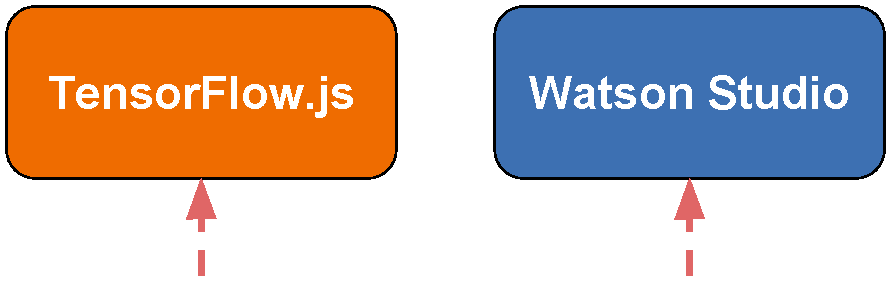
\includegraphics[scale=0.5]{images/kapitel_3/architektur_schematisch.pdf}
    \caption{Schematische Darstellung der Architektur}
    \label{fig:schematische_architektur}
\end{figure}